\documentclass[tikz,border=1pt]{standalone}
\usepackage{amsmath}
\usetikzlibrary{graphs,graphs.standard}
\tikzset{blacknode/.style={shape= circle, fill = black, inner sep = 0pt, outer sep = 0pt, minimum size = 3pt,draw}}
\begin{document}
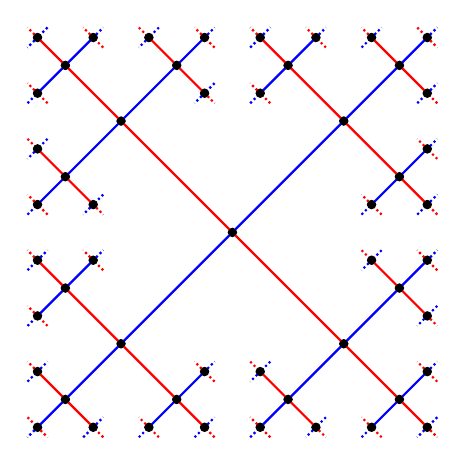
\begin{tikzpicture}[every node/.style=blacknode]
\useasboundingbox (-2.6,-2.6) rectangle (2.6,2.6);
\rotatebox{45}{
\node (0){};
\foreach \i/\j in {E/right ,W/left }{
\node (\i)[\j of = 0,node distance=2cm]{} ;
\node (\i\i)[\j of = \i,node distance=1cm]{} ;
	\node (\i\i N)[above of = \i\i,node distance=0.5cm]{} ;
		\coordinate[above of = \i\i N,node distance=0.18cm] (\i\i NN) ;
		\coordinate[right of = \i\i N,node distance=0.18cm] (\i\i NE) ;
		\coordinate[left of = \i\i N,node distance=0.18cm] (\i\i NW) ;
	\node (\i\i S)[below of = \i\i,node distance=0.5cm]{} ;
		\coordinate[below of = \i\i S,node distance=0.18cm] (\i\i SS) ;
		\coordinate[right of = \i\i S,node distance=0.18cm] (\i\i SE) ;
		\coordinate[left of = \i\i S,node distance=0.18cm] (\i\i SW) ;
	\node (\i\i\i)[\j of = \i\i,node distance=0.5cm]{} ;
		\coordinate[\j of = \i\i\i,node distance=0.18cm] (\i\i\i\i) ;
		\coordinate[above of = \i\i\i,node distance=0.18cm] (\i\i\i N) ;
		\coordinate[below of = \i\i\i,node distance=0.18cm] (\i\i\i S) ;
\node (\i N)[above of = \i,node distance=1cm ]{} ;
	\node (\i NN)[above of = \i N,node distance=0.5cm]{} ;
		\coordinate[above of = \i NN,node distance=0.18cm] (\i NNN) ;
		\coordinate[right of = \i NN,node distance=0.18cm] (\i NNE) ;
		\coordinate[left of = \i NN,node distance=0.18cm] (\i NNW) ;
	\node (\i NW)[left of = \i N,node distance=0.5cm]{} ;
		\coordinate[above of = \i NW,node distance=0.18cm] (\i NWN) ;
		\coordinate[below of = \i NW,node distance=0.18cm] (\i NWS) ;
		\coordinate[left of = \i NW,node distance=0.18cm] (\i NWW) ;
	\node (\i NE)[right of = \i N,node distance=0.5cm]{} ;
		\coordinate[above of = \i NE,node distance=0.18cm] (\i NEN) ;
		\coordinate[below of = \i NE,node distance=0.18cm] (\i NES) ;
		\coordinate[right of = \i NE,node distance=0.18cm] (\i NEE) ;
\node (\i S)[below of = \i,node distance=1cm ]{} ;
	\node (\i SS)[below of = \i S,node distance=0.5cm]{} ;
		\coordinate[below of = \i SS,node distance=0.18cm] (\i SSS) ;
		\coordinate[right of = \i SS,node distance=0.18cm] (\i SSE) ;
		\coordinate[left of = \i SS,node distance=0.18cm] (\i SSW) ;
	\node (\i SW)[left of = \i S,node distance=0.5cm]{} ;
		\coordinate[above of = \i SW,node distance=0.18cm] (\i SWN) ;
		\coordinate[below of = \i SW,node distance=0.18cm] (\i SWS) ;
		\coordinate[left of = \i SW,node distance=0.18cm] (\i SWW) ;
	\node (\i SE)[right of = \i S,node distance=0.5cm]{} ;
		\coordinate[above of = \i SE,node distance=0.18cm] (\i SEN) ;
		\coordinate[below of = \i SE,node distance=0.18cm] (\i SES) ;
		\coordinate[right of = \i SE,node distance=0.18cm] (\i SEE) ;
\graph[edge={thick,color=blue}]{
(0)--(\i )--(\i\i)--(\i\i\i)--[densely dotted](\i\i\i\i),
(\i SWW)--[densely dotted](\i SW)--(\i S)--(\i SE)--[densely dotted](\i SEE),
(\i NWW)--[densely dotted](\i NW)--(\i N)--(\i NE)--[densely dotted](\i NEE),
(\i NNW)--[densely dotted](\i NN)--[densely dotted](\i NNE),
(\i SSW)--[densely dotted](\i SS)--[densely dotted](\i SSE),
(\i\i NW)--[densely dotted](\i\i N)--[densely dotted](\i\i NE),
(\i\i SW)--[densely dotted](\i\i S)--[densely dotted](\i\i SE)
};
\graph[edge={thick,color=red}]{
	(\i SSS)--[densely dotted](\i SS)--(\i S)--(\i)--(\i N)--(\i NN)--[densely dotted](\i NNN),
	(\i\i SS)--[densely dotted](\i\i S)--(\i\i)--(\i\i N)--[densely dotted](\i\i NN),
	(\i\i\i N)--[densely dotted](\i\i\i)--[densely dotted](\i\i\i S),
	(\i NES)--[densely dotted](\i NE)--[densely dotted](\i NEN),
	(\i SES)--[densely dotted](\i SE)--[densely dotted](\i SEN),
	(\i NWS)--[densely dotted](\i NW)--[densely dotted](\i NWN),
	(\i SWS)--[densely dotted](\i SW)--[densely dotted](\i SWN)
};
}
\foreach \i/\j in {N/above ,S/below }{
\node (\i)[\j of = 0,node distance=2cm]{} ;
\node (\i\i)[\j of = \i,node distance=1cm]{} ;
	\node (\i\i W)[left of = \i\i,node distance=0.5cm]{} ;
		\coordinate[above of = \i\i W,node distance=0.18cm] (\i\i WN) ;
		\coordinate[below of = \i\i W,node distance=0.18cm] (\i\i WS) ;
		\coordinate[left of = \i\i W,node distance=0.18cm] (\i\i WW) ;	
	\node (\i\i E)[right  of = \i\i,node distance=0.5cm]{} ;
		\coordinate[above of = \i\i E,node distance=0.18cm] (\i\i EN) ;
		\coordinate[below of = \i\i E,node distance=0.18cm] (\i\i ES) ;
		\coordinate[right of = \i\i E,node distance=0.18cm] (\i\i EE) ;
	\node (\i\i\i)[\j  of = \i\i,node distance=0.5cm]{} ;
		\coordinate[\j of = \i\i\i,node distance=0.18cm] (\i\i\i\i) ;
		\coordinate[right of = \i\i\i,node distance=0.18cm] (\i\i\i E) ;
		\coordinate[left of = \i\i\i,node distance=0.18cm] (\i\i\i W) ;
\node (\i E)[right of = \i,node distance=1cm ]{} ;
	\node (\i EE)[right  of = \i E,node distance=0.5cm]{} ;
		\coordinate[above of = \i EE,node distance=0.18cm] (\i EEN) ;
		\coordinate[below of = \i EE,node distance=0.18cm] (\i EES) ;
		\coordinate[right of = \i EE,node distance=0.18cm] (\i EEE) ;
	\node (\i ES)[below  of = \i E,node distance=0.5cm]{} ;
		\coordinate[below of = \i ES,node distance=0.18cm] (\i ESS) ;
		\coordinate[left of = \i ES,node distance=0.18cm] (\i ESE) ;
		\coordinate[right of = \i ES,node distance=0.18cm] (\i ESW) ;
	\node (\i EN)[above  of = \i E,node distance=0.5cm]{} ;
		\coordinate[above of = \i EN,node distance=0.18cm] (\i ENN) ;
		\coordinate[left of = \i EN,node distance=0.18cm] (\i ENE) ;
		\coordinate[right of = \i EN,node distance=0.18cm] (\i ENW) ;
\node (\i W)[left of = \i,node distance=1cm ]{} ;
	\node (\i WS)[below  of = \i W,node distance=0.5cm]{} ;
		\coordinate[below of = \i WS,node distance=0.18cm] (\i WSS) ;
		\coordinate[left of = \i WS,node distance=0.18cm] (\i WSE) ;
		\coordinate[right of = \i WS,node distance=0.18cm] (\i WSW) ;
	\node (\i WN)[above  of = \i W,node distance=0.5cm]{} ;
		\coordinate[above of = \i WN,node distance=0.18cm] (\i WNN) ;
		\coordinate[left of = \i WN,node distance=0.18cm] (\i WNE) ;
		\coordinate[right of = \i WN,node distance=0.18cm] (\i WNW) ;
	\node (\i WW)[left of = \i W,node distance=0.5cm]{} ;
		\coordinate[above of = \i WW,node distance=0.18cm] (\i WWN) ;
		\coordinate[below of = \i WW,node distance=0.18cm] (\i WWS) ;
		\coordinate[left of = \i WW,node distance=0.18cm] (\i WWW) ;
\graph[edge={thick,color=red}]{
	(0)--(\i )--(\i\i)--(\i\i\i)--[densely dotted](\i\i\i\i),
	(\i ENN)--[densely dotted](\i EN)--(\i E)--(\i ES)--[densely dotted](\i ESS),
	(\i WNN)--[densely dotted](\i WN)--(\i W)--(\i WS)--[densely dotted](\i WSS),
	(\i EES)--[densely dotted](\i EE)--[densely dotted](\i EEN),
	(\i WWS)--[densely dotted](\i WW)--[densely dotted](\i WWN),
	(\i\i ES)--[densely dotted](\i\i E)--[densely dotted](\i\i EN),
	(\i\i WS)--[densely dotted](\i\i W)--[densely dotted](\i\i WN)};
\graph[edge={thick,color=blue}]{
	(\i WWW)--[densely dotted](\i WW)--(\i W)--(\i)--(\i E)--(\i EE)--[densely dotted](\i EEE),
	(\i\i WW)--[densely dotted](\i\i W)--(\i\i)--(\i\i E)--[densely dotted](\i\i EE),
	(\i ENW)--[densely dotted](\i EN)--[densely dotted](\i ENE),
	(\i ESW)--[densely dotted](\i ES)--[densely dotted](\i ESE),
	(\i WNW)--[densely dotted](\i WN)--[densely dotted](\i WNE),
	(\i WSW)--[densely dotted](\i WS)--[densely dotted](\i WSE),
	(\i\i\i E)--[densely dotted](\i\i\i)--[densely dotted](\i\i\i W)};
}
}
\end{tikzpicture}
\end{document}